\documentclass{beamer}
\usetheme{uic}
\usepackage{amsfonts,amsmath,oldgerm,algorithm,algpseudocode}
\usepackage[font=small,labelfont=bf]{caption} % Required for specifying captions to tables and figures
\usepackage{gaml}

\newcommand{\hrefcol}[2]{\textcolor{uihteal}{\href{#1}{#2}}}
\newcommand{\testcolor}[1]{\colorbox{#1}{\textcolor{#1}{test}}~\texttt{#1}}

% Please see Section 18.1 of Beamer User Guide for all the options \usefonttheme provides
\usefonttheme[onlymath]{serif}
% \usefonttheme{serif} % use this if you would like Serif font throughout (and not just for math)


\titlebackground*{assets/usth_lockup_blue.png}

% NOTE 1: The asterisk splits the background image. This option is good
% for logo-based backgrounds. If you use an image based background
% it's recommended to not split it:

% \titlebackground{assets/uic_seo.jpg}

% NOTE 2: If you use a title background that does not have a logo, you might
% want to enable logo in the top left.
% To do that, simply comment out this line
\themecolor{lightnologo}

\title{Modeling and simulation of complex systems}
\subtitle{Project 4: Evacuation}
% This can be adjusted accordingly for longer titles
\setlength{\titleboxwidth}{0.45\textwidth}

\author{\href{mailto:dungvt2440071@usth.edu.vn}{Vu Trung Dung}}
\date{\today}

\begin{document}
\maketitle
\themecolor{lightnologo} % reverts to a logo based theme (if you disabled it for title page)

% enabled after title page creation (i.e. after \maketitle)
\footlinecolor{uicblue}


% ------------------------------------------------
% Question
% ------------------------------------------------
\begin{frame}[fragile]{Question}
% \framesubtitle{}
\textbf{How to better manage the pedestrian evacuation of a population on a beach
in a tsunami context?}

\begin{itemize}
\item flooding will not be modeled by itself
\item just \textbf{the behavior of residents} in the face of the threat.
\end{itemize}
\end{frame}


% ------------------------------------------------
% Modeling
% ------------------------------------------------
\begin{frame}[fragile]{Modeling and Simulation}
\framesubtitle{Situation}
\begin{itemize}
\item People will only evacuate if they have been informed of the flooding. 
\begin{itemize}
    \item We assume that only \textbf{10\% of the population is informed at the beginning of the simulation}.
    \item A person observing someone evacuating
    (at a distance of less than 10m) will have a probability of 0.1 of evacuating in turn.
\end{itemize}
\item \textbf{Not all residents know where to evacuate} and only 10\% will go directly to the shelter.
\item People have multiple mobilities of evacuation: by car, by bike, or on foot.
\end{itemize}
\end{frame}

\begin{frame}[fragile]{Modeling and Simulation}
\framesubtitle{Situation - My extension}
\begin{itemize}
\item \textbf{The knowledge of the evacuation shelter can be transfered across people}.
\begin{itemize}
    \item The knowledge of the evacuation shelter can be shared with 2 people at 10\% probability when they meet each other on the road while evacuating.
    \item When the knowledge is shared, 2 people have 10\% probability to change their evacuation to the closest shelter they're heading to.
\end{itemize}
\end{itemize}
\end{frame}

\begin{frame}[fragile]{Modeling and Simulation}
\framesubtitle{Strategies to aware of flooding}

Different strategies of aware of flooding to the 10\% of the population:
\begin{itemize}
    \item random.
    \item furthest from the shelter.
    \item closest to the shelter.
\end{itemize}

\textbf{Find the most effective} of these strategies in terms of:
\begin{itemize}
    \item number of evacuees.
    \item evacuation time.
    \item time for the total evacuation/time spent on the roads.
\end{itemize}
\end{frame}


% \begin{frame}[fragile]{Modeling and Simulation}
% \framesubtitle{Parameters}

% \begin{itemize}
%     \item initial population.
%     \item the alert time before the flooding.
% \end{itemize}

% \end{frame}


% ------------------------------------------------
% GIS DATA
% ------------------------------------------------
\begin{frame}[fragile]{GIS Data}
% \framesubtitle{The }



\begin{columns}
\begin{column}{0.5\textwidth}
In this project, we will use the GIS data of Hanoi and the Red River in the previous exercises.

\end{column}

\begin{column}{0.5\textwidth}
    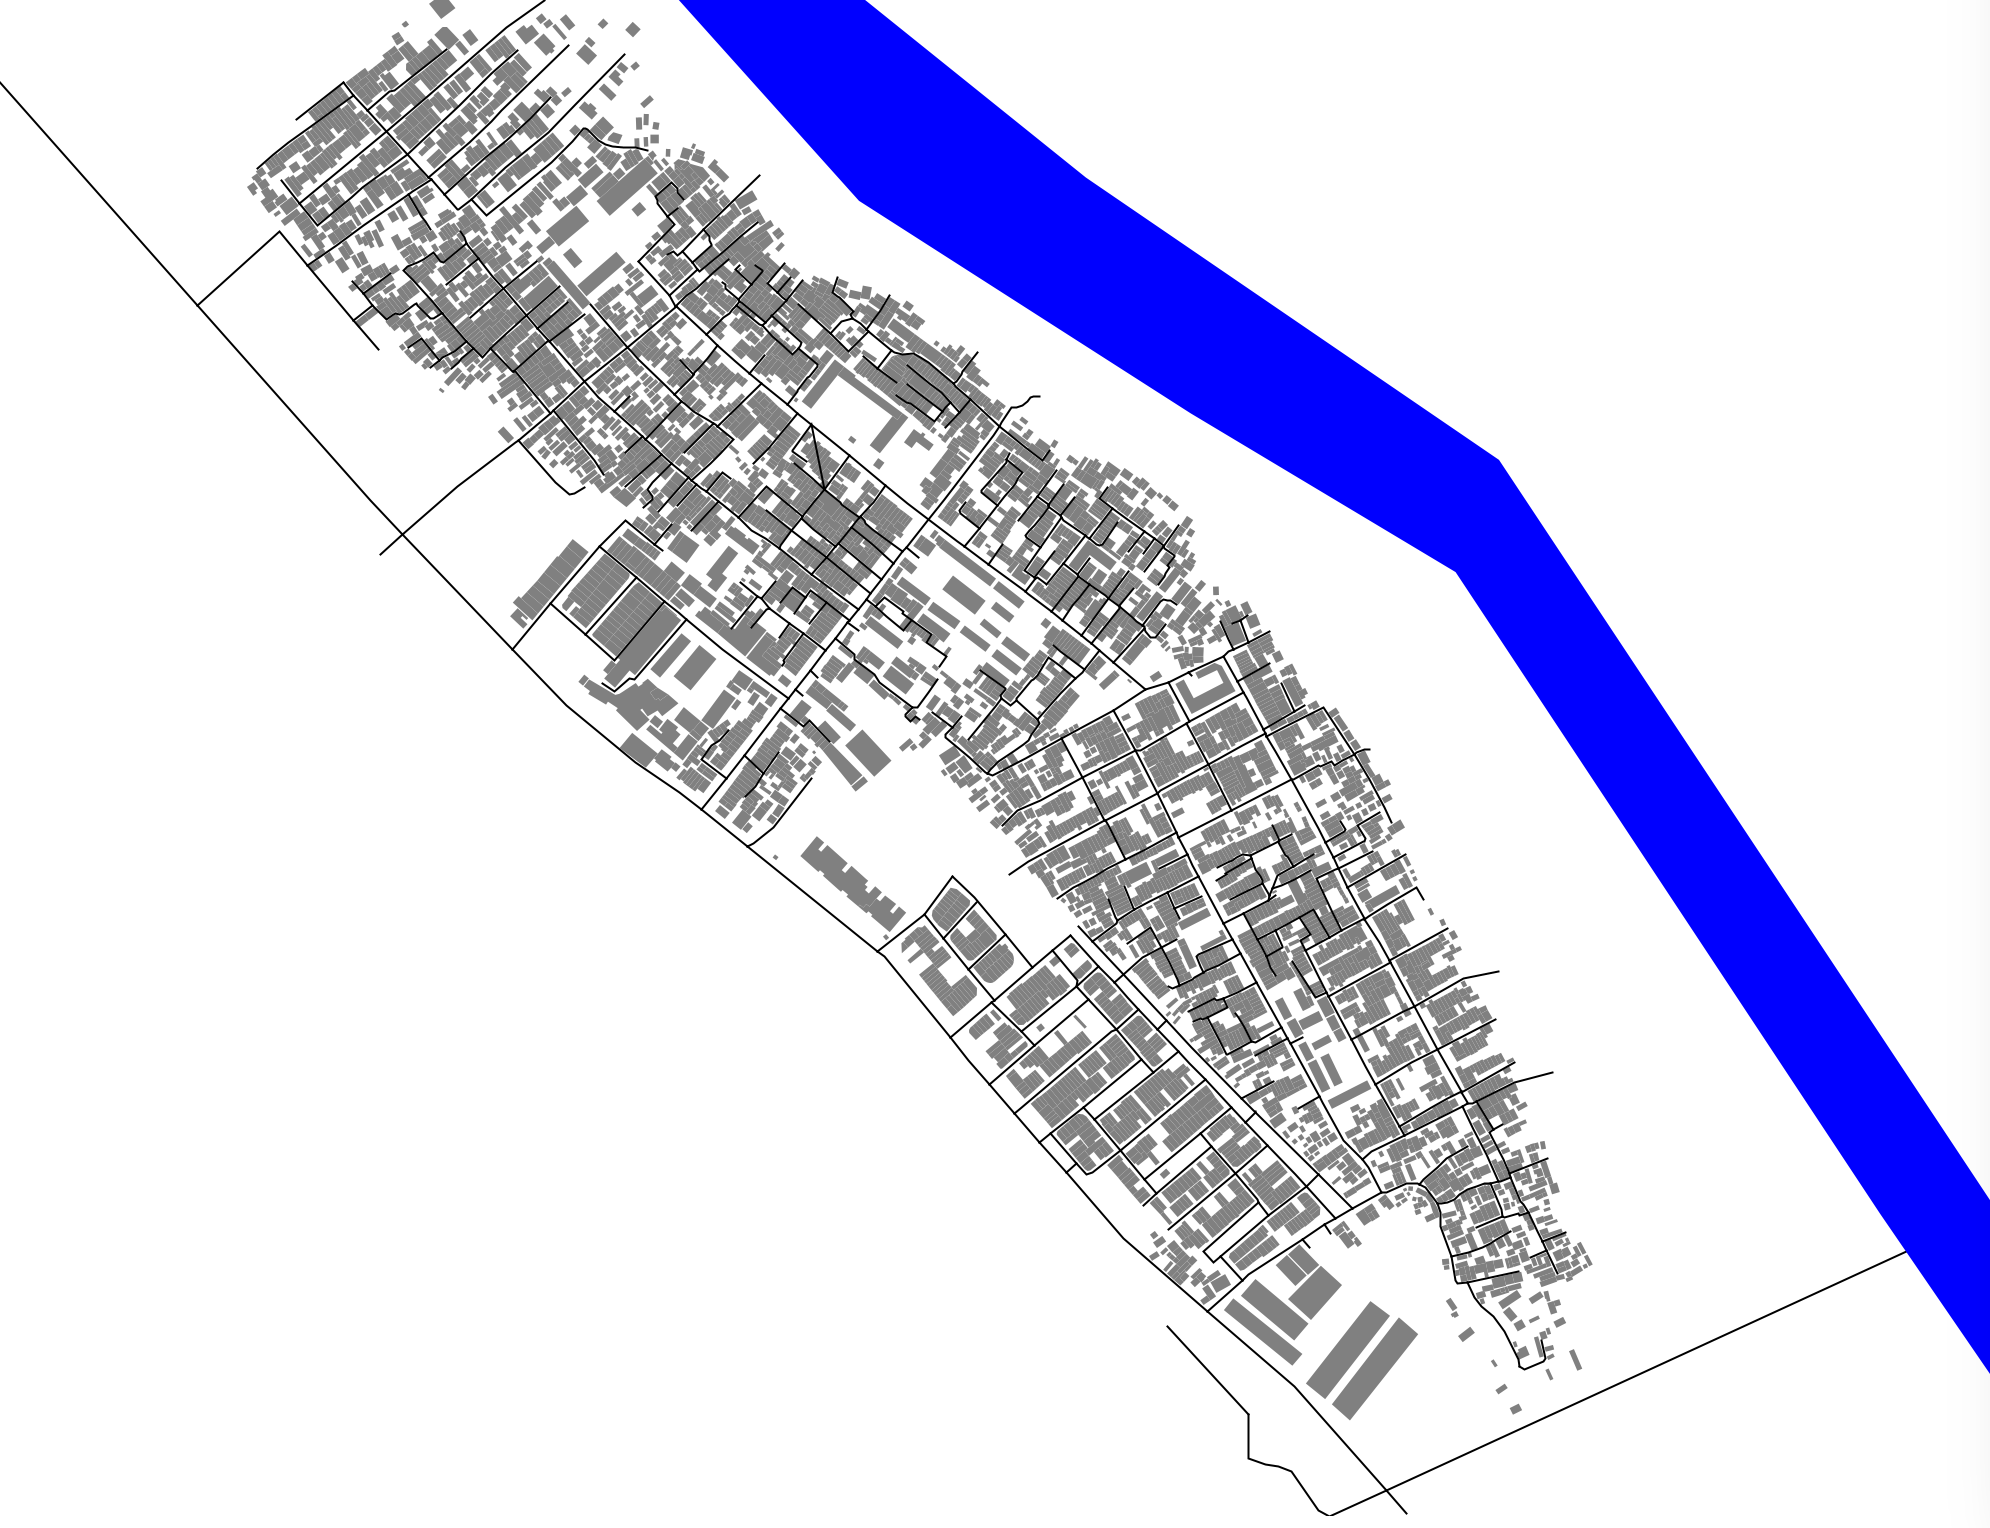
\includegraphics[width=\textwidth]{img/GIS-map-hanoi-red-river-original.png}
    \captionof{figure}{GIS map for the simulation}
\end{column}
\end{columns}

\end{frame}


% ------------------------------------------------
% Implementation - Extensions
% ------------------------------------------------
\begin{frame}[fragile]{Implementation (GAMA)}
\framesubtitle{Extensions}

\begin{itemize}
    \item \textbf{Extensions 0}: GIS map, population, evacuation shelter, roads, flooding simulation, etc.
    \item \textbf{Extensions 1}: The evacuating behavior of the population.
    \item \textbf{Extensions 2}: Multimobility of population (car, bike, foot).
    \item \textbf{My Extensions}: The knowledge of the evacuation shelter can be transfered across people.
    \item \textbf{Extensions 3}: Experiment and analyze the effectiveness of different strategies of aware of flooding.
\end{itemize}

\end{frame}


% ------------------------------------------------
% Implementation - Extensions 0
% ------------------------------------------------
\begin{frame}[fragile]{Implementation: Extensions 0}
\framesubtitle{The Map}

\begin{columns}
\begin{column}{0.5\textwidth}
\begin{itemize}
    \item Hanoi and Red River GIS map.
    \item The \textbf{Evacuation Shelter} is the N largest building in the map (red color). The sample code:

\begin{lstlisting}[style=GAML]
evacuations <- 8 first (
    building sort_by -each.shape.area
);
ask evacuations {
    self.is_evacuation <- true;
}
\end{lstlisting}

\end{itemize}

\end{column}

\begin{column}{0.5\textwidth}
    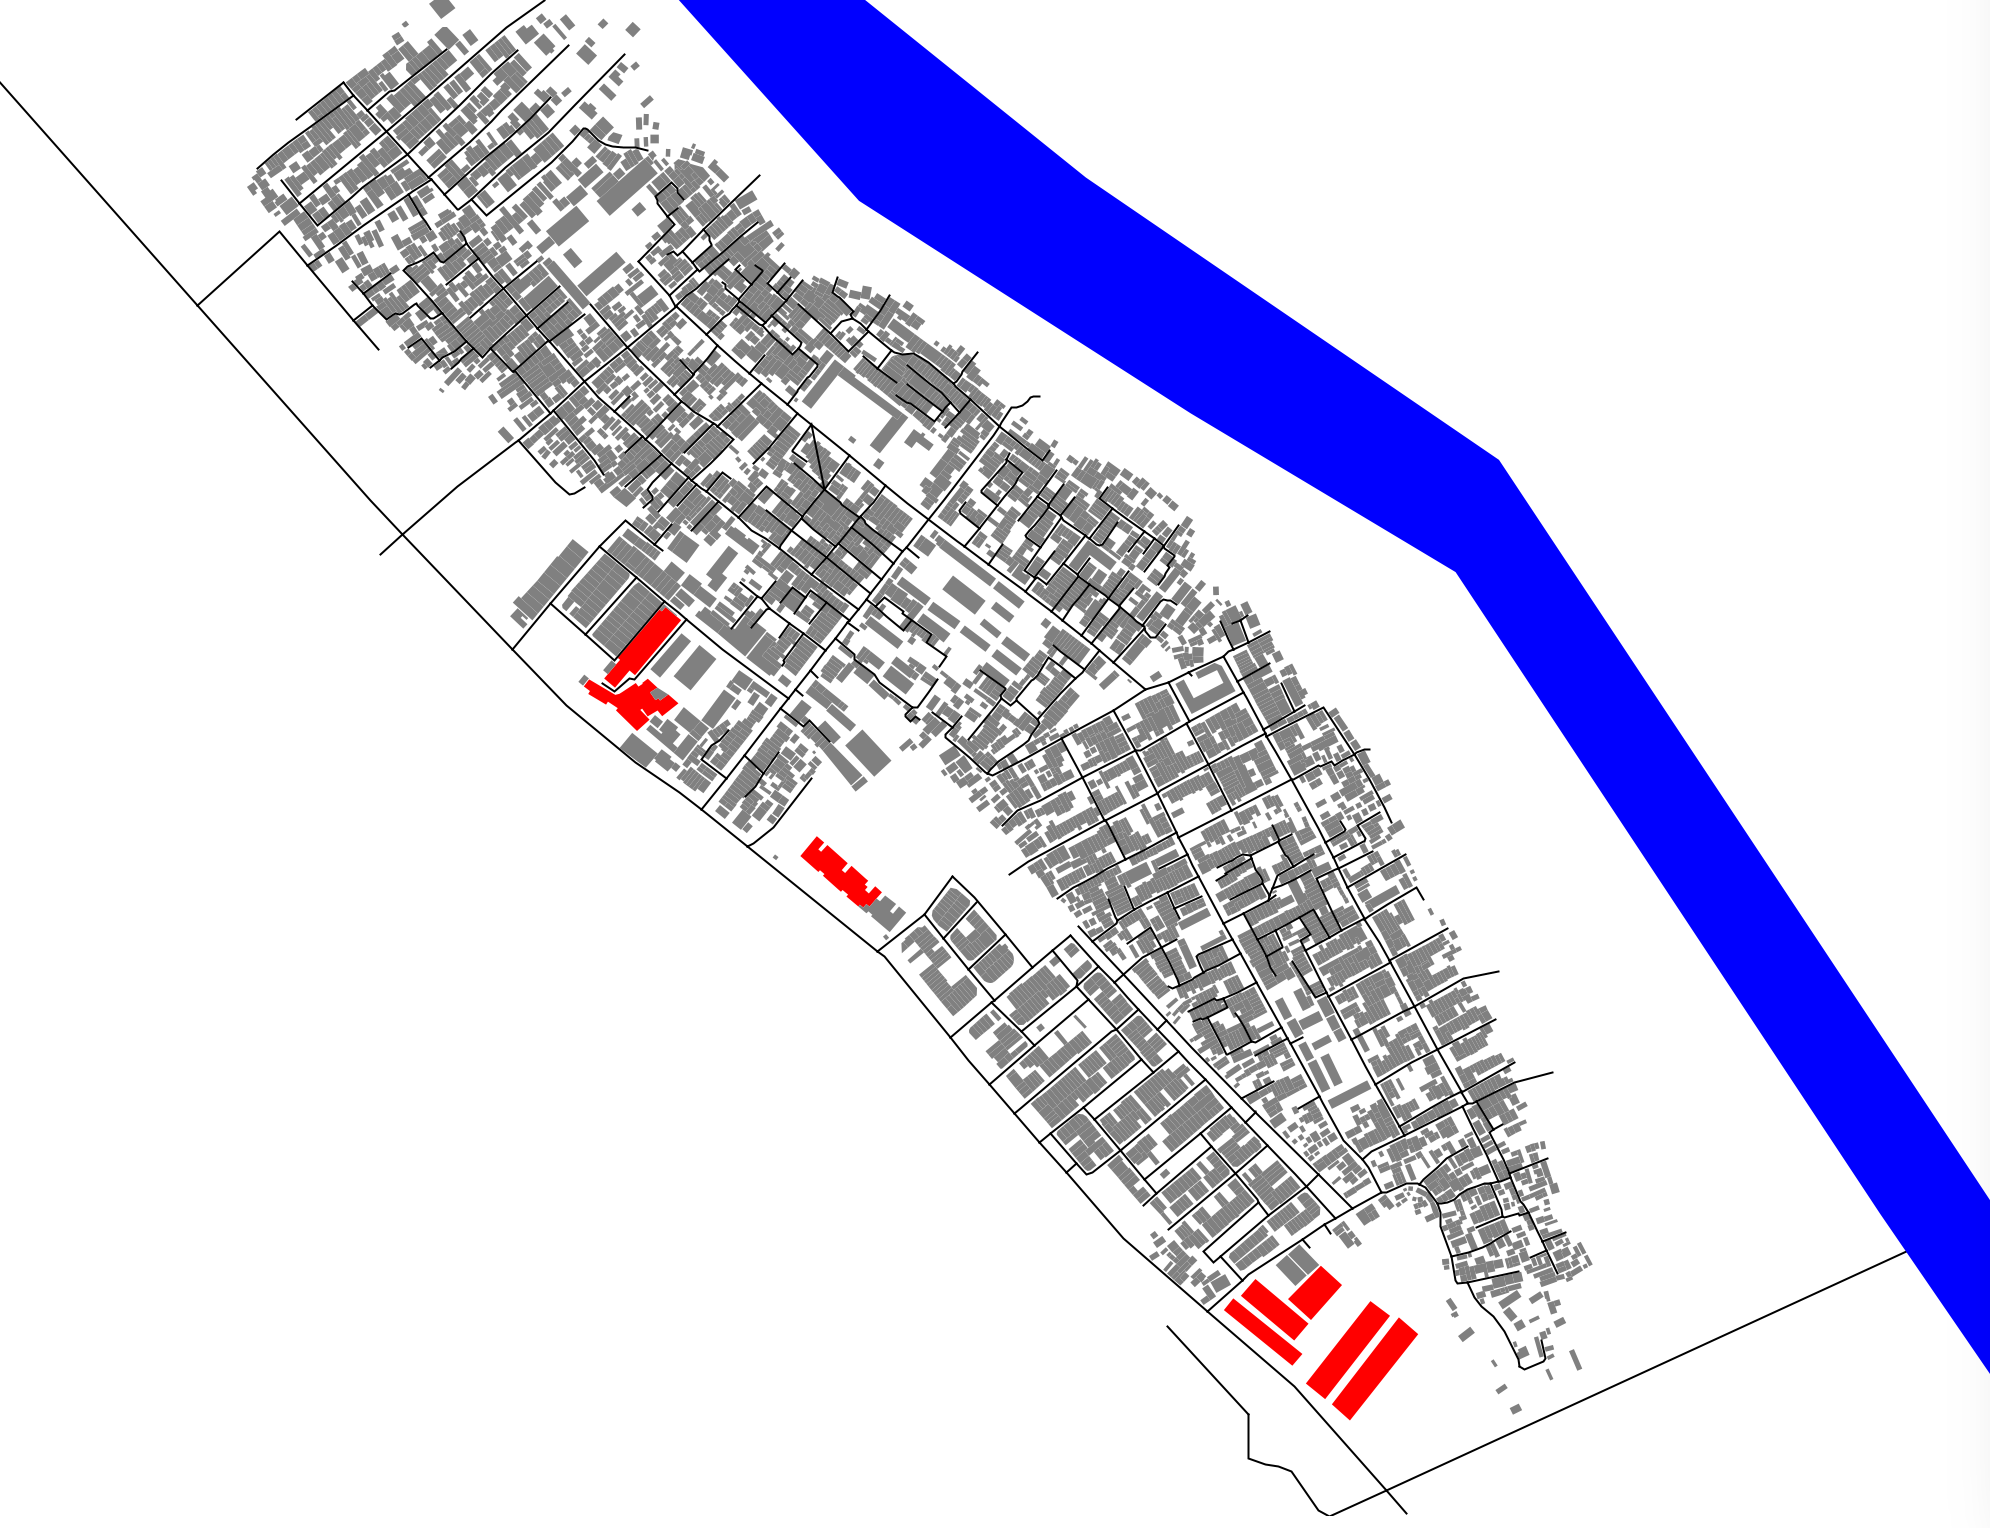
\includegraphics[width=\textwidth]{img/GIS-map-hanoi-red-river.png}
    \captionof{figure}{Map and Evacuation Representation}
\end{column}
\end{columns}

\end{frame}


% ------------------------------------------------
% Implementation - Extensions 0
% ------------------------------------------------
\begin{frame}[fragile]{Implementation: Extensions 0}
\framesubtitle{Species}

\begin{itemize}
    \item \textbf{People}: the inhabitants of the city.
    \item \textbf{Evacuation Shelter}: the shelter for evacuation.
    \item \textbf{Road}: the road for evacuation.
    \item \textbf{Building}: the building in the city.
    \item \textbf{Flooding}: the flooding area.
\end{itemize}

\end{frame}

% ------------------------------------------------
% Implementation - Extensions 0
% ------------------------------------------------
\begin{frame}[fragile]{Implementation: Extensions 0}
\framesubtitle{Species - Flooding}

Implement the flooding simulation with the following parameters:
\begin{itemize}
    \item \textbf{Flooding date}: the start date of flooding.
    \item \textbf{Grow rate and flooding speed}: how fast the flooding grows.
\end{itemize}

\begin{lstlisting}[style=GAML]
float grow_rate <- 0.5;
float flooding_speed <- 0.1;

reflex expand when: flooding_date <= current_date and every(1#m) 
{
    grow_rate <- grow_rate + flooding_speed;
    shape <- shape + grow_rate;
}
\end{lstlisting}

\end{frame}

% ------------------------------------------------
% Implementation - Extensions 1
% ------------------------------------------------
\begin{frame}[fragile]{Implementation: Extensions 1}
\framesubtitle{Species - Initial Population}

\begin{columns}
\begin{column}{0.7\textwidth}
\begin{itemize}
    \item No more 5 people in a building (customizable).
    \item People are located randomly in the city except the evacuation shelters.

\begin{lstlisting}[style=GAML]
create inhabitant number: 1000 {
    location <- any_location_in(one_of(building));
    
    ask any(building where (!each.is_evacuation and length(each.inhabitants) < max_n_inhabitants_in_building)) {
        self.inhabitants << myself;
        myself.location <- any_location_in(self);
    }
}
\end{lstlisting}

\end{itemize}

\end{column}

\begin{column}{0.3\textwidth}
    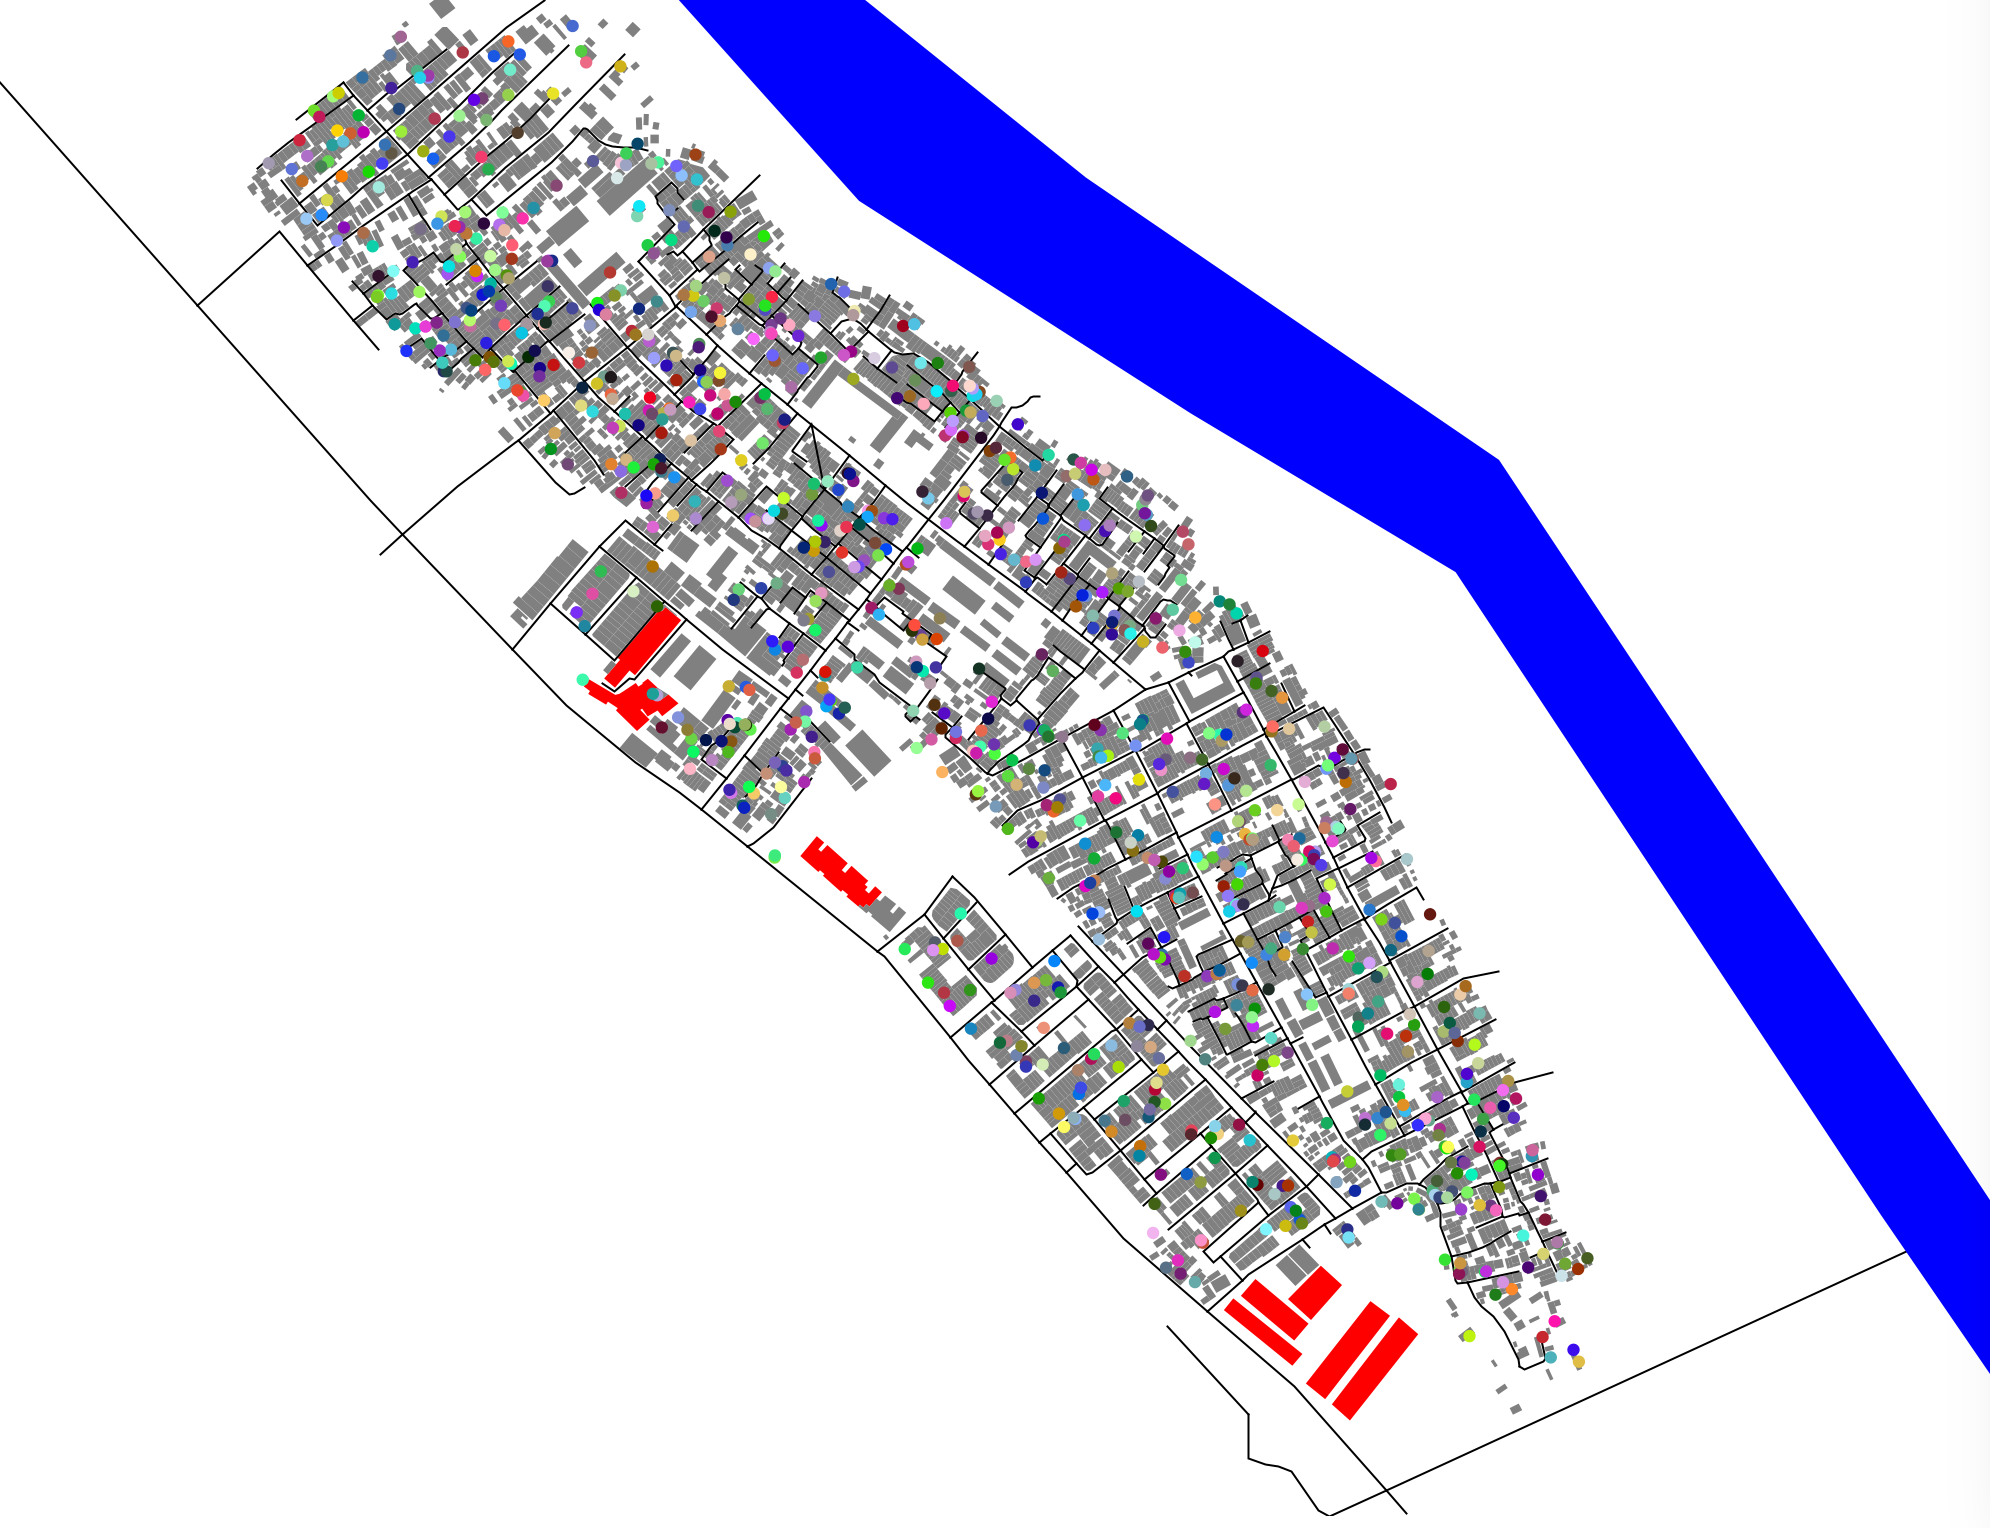
\includegraphics[width=\textwidth]{img/People-in-building.png}
    \captionof{figure}{People in building}
\end{column}
\end{columns}

\end{frame}


% ------------------------------------------------
\begin{frame}[fragile]{Implementation: Extensions 1}
\framesubtitle{Species - Aware of Flooding}

\begin{itemize}
    \item Only 10\% of the population know about the shelter at the beginning.
    
\begin{lstlisting}[style=GAML]
ask (int(percentage_of_people_known_shelter * length(inhabitant))) among inhabitant {
    target_shelter <- evacuations closest_to self;
}
\end{lstlisting}

    \item Only 10\% of the population is informed about the flooding.
\begin{lstlisting}[style=GAML]
reflex flooding_announce when: flooding_inform_date <= current_date and !flooding_is_informed {		
    flooding_is_informed <- true;
    
    ask (int(percentage_of_people_are_informed * length(inhabitant))) among inhabitant {
        is_evacuating <- true;
    }
} 
\end{lstlisting}

\end{itemize}

\end{frame}


% ------------------------------------------------
\begin{frame}[fragile]{Implementation: Extensions 1}
\framesubtitle{Species - People behavior}

\begin{lstlisting}[style=GAML]
reflex observe_evaculating when: !is_evacuating and flip(percentage_of_following_evaculating) every(5#s) {
    if !empty((inhabitant where each.is_evacuating) at_distance 20#m)  {
        is_evacuating <- true;
    }
}

reflex find_shelter when: target = nil and is_evacuating every(5#s) {
    building target_building <- target_shelter;
    if (target_building = nil) {
        target_building <- one_of(building - visited_buildings);
    }
    visited_buildings << target_building;
    target <- any_location_in(target_building);
}
\end{lstlisting}


\end{frame}


% ------------------------------------------------
\begin{frame}[fragile]{Implementation: Extensions 1}
\framesubtitle{Species - Evacuation behaviour}

\begin{lstlisting}[style=GAML]
reflex evacuating_people when: is_evacuation every(5#s) {
    ask (inhabitant at_distance 20#m) {
        target_shelter <- myself;
        target <- any_location_in(target_shelter);
    }
    ask (inhabitant at_distance 0.5#m) {
        number_evacuted_people <- number_evacuted_people + 1;
        do die;
    }
}
\end{lstlisting}


\end{frame}


% ------------------------------------------------
% Implementation - Extensions 2
% ------------------------------------------------
\begin{frame}[fragile]{Implementation: Extensions 2}
\framesubtitle{Multimobility of population}

Initialize inhabitants with different evacuation modalities:
\begin{lstlisting}[style=GAML]
int count <- 0;
create inhabitant number: nb_of_people {
    count <- count + 1;
    if count < nb_of_people * percentage_of_car {
        traffic_weight <- traffic_weight_factor * 5;
        speed <- 10 * pedestrians_speed;
    } else if count < nb_of_people * (percentage_of_car + percentage_of_bike) {
        traffic_weight <- traffic_weight_factor * 2.5;
        speed <- 8.5 * pedestrians_speed;
    } else {
        traffic_weight <- traffic_weight_factor;
        speed <- pedestrians_speed;
    }
}
\end{lstlisting}

\end{frame}

% ------------------------------------------------
\begin{frame}[fragile]{Implementation: Extensions 2}
\framesubtitle{Road and Traffic Weight}

\begin{itemize}
    \item Calculate the traffic weight of each road.

    \begin{lstlisting}[style=GAML]
float capacity <- 1 + shape.perimeter/10;
float total_traffic_weight <- 0.0 
    update: sum((inhabitant at_distance 1) collect each.traffic_weight);
float speed_rate <- 1.0 
    update: exp(-total_traffic_weight/capacity) min: 0.1;
\end{lstlisting}

    \item Update the weight of the road network.

\begin{lstlisting}[style=GAML]
reflex update_speed { 
    road_weights <- road as_map (each::each.shape.perimeter / each.speed_rate);
}
\end{lstlisting}
\end{itemize}
\end{frame}


% ------------------------------------------------
\begin{frame}[fragile]{Implementation: Extensions 2}
\framesubtitle{Representation of different evacuation mobilities}

\begin{columns}
\begin{column}{0.4\textwidth}

\begin{itemize}
    \item \textbf{Car}: big squares.
    \item \textbf{Bike}: triangle.
    \item \textbf{Foot}: small circle.
\end{itemize}
\end{column}

\begin{column}{0.6\textwidth}
    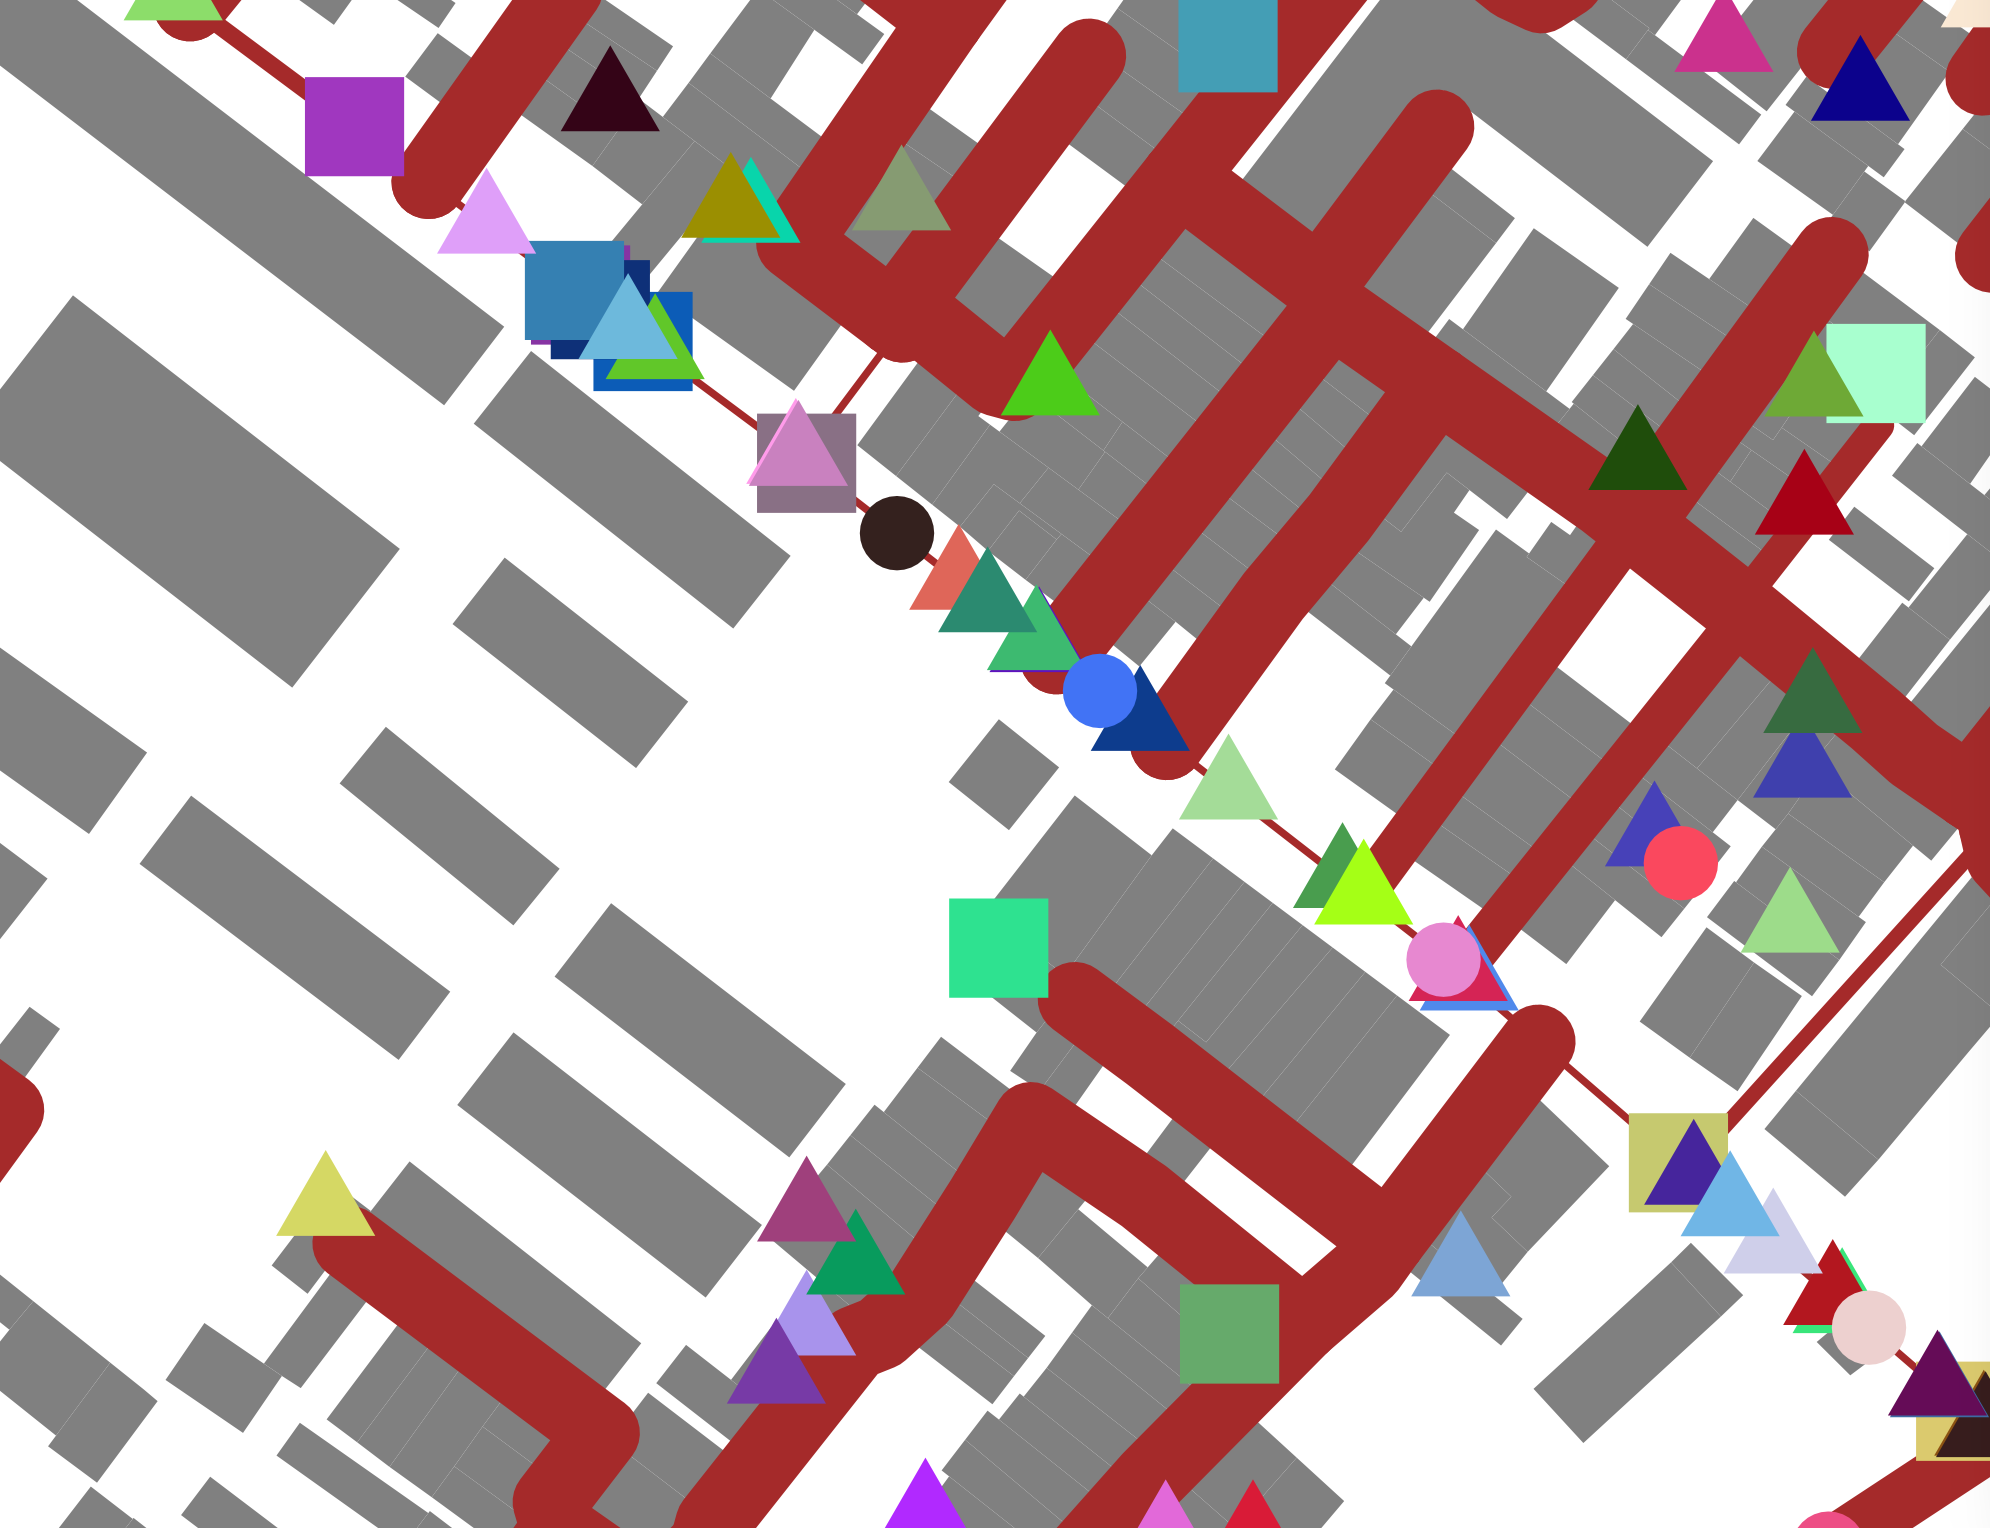
\includegraphics[width=\textwidth]{img/Mobilities.png}
    \captionof{figure}{Representation of mobilities}
\end{column}

\end{columns}

\end{frame}


% ------------------------------------------------
% Implementation - My Extensions
% ------------------------------------------------
\begin{frame}[fragile]{Implementation: My Extensions}
\framesubtitle{Transfer knowledge of evacuation shelter}
    
\begin{lstlisting}[style=GAML]
reflex share_shelter when: is_evacuating and every(5#s) 
        and flip(percentage_of_share_shelter) {

    ask inhabitant at_distance 10#m {
        building shelter <- [myself.target_shelter, self.target_shelter] closest_to myself;
        if (shelter != nil) {
            is_evacuating <- true;
            target_shelter <- shelter;
            target <- any_location_in(shelter);
            myself.target_shelter <- shelter;
            myself.target <- any_location_in(shelter);
        }
    }
}
\end{lstlisting}
    
\end{frame}

% ------------------------------------------------
% Implementation - Extensions 3 - Random
% ------------------------------------------------
\begin{frame}[fragile]{Implementation: Extensions 3}
\framesubtitle{Trategies Implementation (1)}
    
\begin{lstlisting}[style=GAML]
reflex flooding_announce when: flooding_inform_date <= current_date and !flooding_is_informed {		
    flooding_is_informed <- true;
    
    int nb_informing_people <- int(percentage_of_people_are_informed * length(inhabitant));
    
    if (initial_inform_strategy = "random") {
        ask nb_informing_people among inhabitant {
            is_evacuating <- true;
        }
    } else if (initial_inform_strategy = "furthest") {
        ...
} 
\end{lstlisting}

\end{frame}

% ------------------------------------------------
% Implementation - Extensions 3 - Furthest
% ------------------------------------------------
\begin{frame}[fragile]{Implementation: Extensions 3}
\framesubtitle{Trategies Implementation (2)}
    
\begin{lstlisting}[style=GAML]
reflex flooding_announce when: flooding_inform_date <= current_date and !flooding_is_informed {		
    ...
    } else if (initial_inform_strategy = "furthest") {
        ask inhabitant {
            distance_to_shelter <- max(evacuations collect distance_to(self, each));
        }
        ask nb_informing_people first (inhabitant sort_by -each.distance_to_shelter) {
            is_evacuating <- true;
        }
    } else {
    ...
} 
\end{lstlisting}

\end{frame}



% ------------------------------------------------
% Implementation - Extensions 3 - Furthest
% ------------------------------------------------
\begin{frame}[fragile]{Implementation: Extensions 3}
\framesubtitle{Trategies Implementation (3)}
    
\begin{lstlisting}[style=GAML]
reflex flooding_announce when: flooding_inform_date <= current_date and !flooding_is_informed {		
    ...
    } else {
        ask inhabitant {
            distance_to_shelter <- min(evacuations collect distance_to(self, each));
        }
        ask nb_informing_people first (inhabitant sort_by each.distance_to_shelter) {
            is_evacuating <- true;
        }
    }
} 
\end{lstlisting}

\end{frame}

% ------------------------------------------------
% Experiment - Comparison
% ------------------------------------------------
\begin{frame}[fragile]{Experiment}
\framesubtitle{Comparison}

% Setup the randomness.
% A grid of experiments to compare the effectiveness of different strategies of aware of flooding. Y is the strategy, X is the parameter (initial population, alert time before the flooding, transfer knowlege on/off).
% Find the sensitivity of the parameters.

\end{frame}

% ------------------------------------------------
% Experiment - Batch exploration
% ------------------------------------------------
\begin{frame}[fragile]{Experiment}
\framesubtitle{Batch exploration}

% Batch exploration to find the most effective strategy.

\end{frame}

\backmatter
\end{document}
